\documentclass[•]{article}
\usepackage[]{amsmath}
\usepackage{tikz}
\usepackage{pgfplots}

\title{Revisão P1 Pesquisa e Ordenação de Dados\\Giancarlo}
\author{Erickson G. Müller}

\begin{document}
	\maketitle
	\section{Conteúdos}
		\begin{enumerate}
			\item Complexidade de Algoritmos
			\item Bubble Sort
			\item Selection Sort
			\item Insertion Sort
			\item Merge Sort
			\item Quick Sort
			\item Heap Sort
		\end{enumerate}
	\newpage
	\section{Métodos de Ordenação}
		\subsection{Ordenação Estável}
			Preserva a ordem relativa dos elementos que possuem o mesmo valor para a chave de ordenação. Composto por mais de uma chave.
		\subsection{Ordenação Não Estável}
		\subsection{In place/In situ}
			Os valores são permutados dentro da própria estrutura do vetor, não havendo necessidade de duplicar a memória.
		\subsection{Ordenação Interna}
			O arquivo a ser ordenado cabe dentro da memória principal (RAM), qualquer registro pode ser acessado imediatamente.
		\subsection{Ordenação Externa}
			O arquivo a ser ordenado não cabe na memória principal(RAM), os registros são acessados sequencialmente ou em grandes blocos.
	\section{Bubble Sort}
		Compara pares de elementos adjacentes, dois de cada vez, colocando os dois em ordem. Se o elemento da esquerda é maior que o da direita, troca-os de posição.\\
		São realizadas até $n-1$ iterações, em que cada uma delas:
		\begin{enumerate}
			\item Percorre a lista a partir do início
			\item Compara cada elemento com o seu sucessor
			\item Troca os elementos caso o sucessor seja menor que o elemento comparado
		\end{enumerate}
		O objetivo de cada iteração é levar o maior elemento para o final do vetor. Portanto, a parte ordenada fica à direita.\\
		Complexidade: $O(n^2)$\\	
		Memória: \textit{in place}(constante)\\
		Estável.\\
		Número de comparações: $\dfrac{n^2 - n}{2}$
		
	\section{Selection Sort}
		Consiste em identificar o menor valor e trocar com o elemento de menor índice, e assim sucessivamente até que reste apenas o elemento de último índice. Durante o processo, dividir a lista em parte ordenada (à esquerda) e parte não ordenada (à direita).\\
		São realizadas $n-1$ iterações, em que cada uma delas:
		\begin{enumerate}
			\item Seleciona o menor elemento da parte não ordenada.
			\item Troca-o com o elemento de menor posição da parte não ordenada.
			\item Incorpora esse elemento na parte ordenada.
		\end{enumerate}
		Complexidade: $O(n^2)$ em \textbf{todos} os casos.\\
		Memória: \textit{in place}(constante).\\
		Não é estável.\\
		Recomendado para registros muito grandes, onde o custo da movimentação supera o custo das comparações (nessa ordenação, são feitas no máximo $n$ trocas).
	\section{Insertion Sort}
		Divide-se o vetor em parte ordenada (à esquerda) e parte não ordenada (à direita). A parte não ordenada funciona como uma fila para entrar na parte ordenada, o primeiro elemento da parte ordenada é removido e posicionado no local certo da parte ordenada, movendo todos os elementos que forem maiores que ele uma casa para a direita.\\
		São realizadas até $n-1$ iterações, em que cada uma delas:
		\begin{enumerate}
			\item Pega o primeiro elemento da parte não ordenada.
			\item Verifica qual seria sua posição de inserção na parte ordenada.
			\item Desloca os elementos maiores para a direita até encontrar a posição.
			\item P é inserido à esquerda do último elemento movido.
		\end{enumerate}
		Complexidade: $O(n^2)$ quando a lista for inversamente ordenada, pois cada iteração requer que todos os elementos sejam deslocados.\\
		Memória: \textit{in place}.\\
		Estável.\\
		Número de comparações: $\dfrac{n^2-n}{2}$ (pior caso) ou $n-1$ (melhor caso).\\
		Eficiente para listas quase ordenadas, ou quando for necessário inserir um elemento numa lista já ordenada.\\
		Com a complexidade $O(n^2)$, o algoritmo é muito mais lento que o selection sort, pois executa o mesmo número de comparações, mas com mais trocas. Com a complexidade $O(n)$, o algoritmo é muito mais rápido que o selection sort.		
		
	\section{Merge Sort}	
		\begin{center}
			Dividir em elementos ordenados  e depois intercalar na ordem correta
		\end{center}
	\section{Quick Sort}
		Não precisa de memória extra(in-place).\\
		Em tese $n \log n$\\
		Pior caso = $n^2$(Quando já está ordenado).\\
		Algoritmo de \textbf{Ordenação Instável}\\
		Divisão e consquista.\\
		i = posição que estou fazendo a comparação\\
		k = 
		se $i>pivo \to$ k fica parado e i vai para o próximo elemento\\
		se $pivo>i \to$ elemento k troca com i, k e i vão para o próximo elemento\\
		Quando i chega na posição do pivô $\to$ trocar o k pelo pivô
		\subsection{Regras}
		Se o Elemento for maior que o pivô	: i anda, k fica parado\\
		Se o Elemento for menor que o pivô: i anda, k anda\\
		Se o Elemento for menor que a posição do k: troca elemento com o k, k anda
		Passos:
		\begin{enumerate}
			\item Escolher o pivô (tradicionalmente o último elemento);
			\item Particionamento (posicionar em relação ao pivô)\\
			
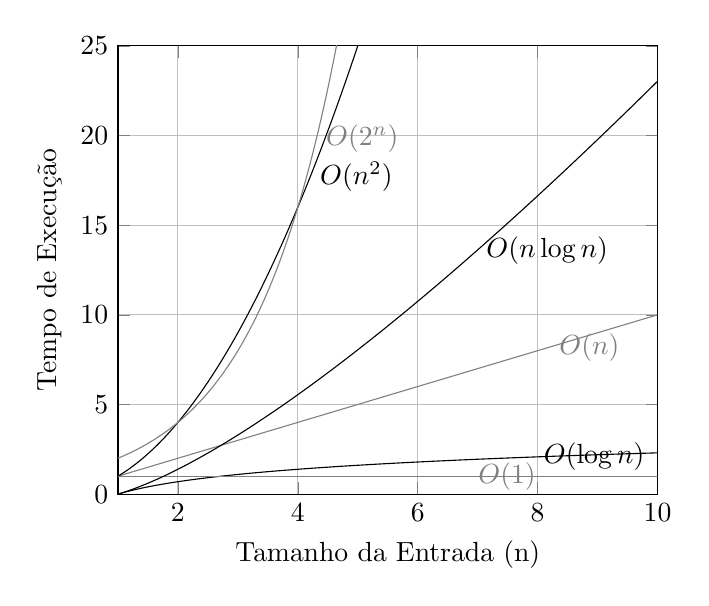
\begin{tikzpicture}
    \begin{axis}[
        xlabel={Tamanho da Entrada (n)},
        ylabel={Tempo de Execução},
        xmin=1, xmax=10,
        ymin=0, ymax=25,
        grid=both,
        legend pos=north west
    ]

    \addplot[domain=1:10, samples=100, color=gray]{x} node[pos=0.8,right]{$O(n)$};
    \addplot[domain=1:5, samples=100, color=black]{x^2} node[pos=0.7,right]{$O(n^2)$};
    \addplot[domain=1:10, samples=100, color=black]{ln(x)} node[pos=0.78,right]{$O(\log n)$};
    \addplot[domain=1:10, samples=100, color=gray]{1} node[pos=0.65,right]{$O(1)$};
    \addplot[domain=1:10, samples=100, color=black]{x* ln(x)} node[pos=0.6,right]{$O(n \log n)$};
    \addplot[domain=1:5, samples=100, color=gray]{2^x} node[pos=0.6,right]{$O(2^n)$};
    % Adicione mais curvas conforme necessário:
    %\addplot[domain=1:10, samples=100, color=black]{2^x} node[pos=0.8,right]{$O(2^n)$};
    %\addplot[domain=1:10, samples=100, color=black]{x*ln(x)} node[pos=0.8,right]{$O(n \log n)$};

    \end{axis}
\end{tikzpicture}
			
			
		\end{enumerate}
	\section{Counting Sort}
		Só serve para ordenação de inteiros positivos, Complexidade N. Ruim para economizar memória (questão do Count = K+1). Ver counting.md
	\section{Radix Sort}
		O counting do radix é de apenas 10 posições. Conta-se os dígitos do numeral.
		
\end{document}
